\documentclass[tikz,border=7pt]{standalone}
\usepackage{iftex}
\ifPDFTeX
  \PackageError{matrix-figure}{This figure requires XeTeX or Tectonic}{Compile with xelatex or tectonic.}
\fi
\usepackage{fontspec}
\usepackage{xeCJK}
\usepackage{amsmath}
\usepackage{unicode-math}
\usepackage{xcolor}
\usepackage{tikz}
\usetikzlibrary{arrows.meta,positioning}

\providecommand{\FigureUseLocalFonts}{0}
\ifnum\FigureUseLocalFonts=1
  \setmainfont{NotoSansCJKtc-Regular.otf}[Path=\FigureSansFontPath]
  \setsansfont{NotoSansCJKtc-Regular.otf}[Path=\FigureSansFontPath,BoldFont=NotoSansCJKtc-Bold.otf]
  \setCJKmainfont{NotoSansCJKtc-Regular.otf}[Path=\FigureSansFontPath]
  \setCJKsansfont{NotoSansCJKtc-Regular.otf}[Path=\FigureSansFontPath,BoldFont=NotoSansCJKtc-Bold.otf]
  \setmathfont{STIXTwoMath.otf}[Path=\FigureMathFontPath]
\else
  \setmainfont{Noto Sans CJK TC}
  \setsansfont{Noto Sans CJK TC}
  \setCJKmainfont{Noto Sans CJK TC}
  \setCJKsansfont{Noto Sans CJK TC}
  \setmathfont{STIX Two Math}
\fi

\definecolor{FigureInk}{HTML}{253142}
\definecolor{PanelFill}{gray}{0.96}
\definecolor{RowShade}{gray}{0.86}
\definecolor{ColumnShade}{gray}{0.74}
\definecolor{ResultShade}{gray}{0.58}
\definecolor{FocusShade}{gray}{0.68}
\definecolor{GuideShade}{gray}{0.80}

\newcommand{\MatrixCell}[2]{%
  \tikz[baseline=(value.base)]{\node[fill=#1,rounded corners=0.4pt,inner sep=2.2pt,
    minimum width=1.35em,minimum height=1.35em] (value) {$#2$};}%
}
\newcommand{\RowCell}[1]{\MatrixCell{RowShade}{#1}}
\newcommand{\ColumnCell}[1]{\MatrixCell{ColumnShade}{#1}}
\newcommand{\ResultCell}[1]{\MatrixCell{ResultShade}{#1}}
\newcommand{\FocusCell}[1]{\MatrixCell{FocusShade}{#1}}

\tikzset{
  figure/.style={font=\sffamily,text=FigureInk,>={Stealth[length=3.5mm,width=2.5mm]}},
  panel/.style={draw=FigureInk,line width=0.9pt,rounded corners=1.5mm,fill=PanelFill,align=center},
  flow/.style={-{Stealth},line width=1.05pt,draw=FigureInk},
}


\begin{document}
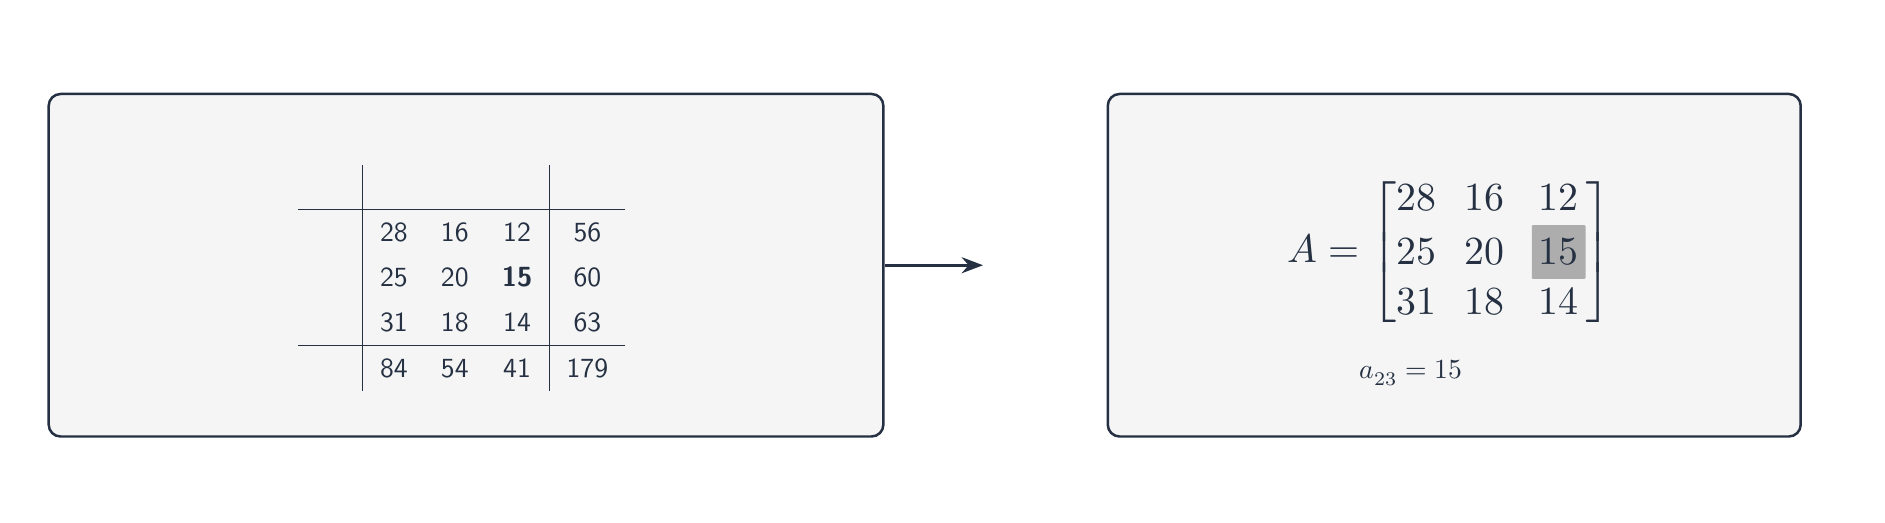
\begin{tikzpicture}[figure]
  \node[font=\bfseries\Large,align=center,text width=23cm] at (11.5,6.05)
    {資料表的列、行標籤決定矩陣中每個元素的意義};

  \node[panel,minimum width=10.6cm,minimum height=4.35cm] (table) at (5.45,3.15) {%
    \begin{minipage}{9.9cm}\centering
      \textbf{通勤方式資料表}\\[8pt]
      \renewcommand{\arraystretch}{1.35}
      \begin{tabular}{c|ccc|c}
        & 公車 & 步行 & 單車 & 班級合計\\ \hline
        甲班 & 28 & 16 & 12 & 56\\
        乙班 & 25 & 20 & \textbf{15} & 60\\
        丙班 & 31 & 18 & 14 & 63\\ \hline
        方式合計 & 84 & 54 & 41 & 179
      \end{tabular}
    \end{minipage}
  };

  \draw[flow] (table.east) -- ++(1.25,0);
  \node[panel,minimum width=8.8cm,minimum height=4.35cm] (matrix) at (18.0,3.15) {%
    \begin{minipage}{8.1cm}\centering
      \textbf{固定標籤順序後的矩陣}\\[10pt]
      \Large$A=\begin{bmatrix}
        28&16&12\\
        25&20&\FocusCell{15}\\
        31&18&14
      \end{bmatrix}$\\[10pt]
      \normalsize$a_{23}=15$：乙班使用單車的人數
    \end{minipage}
  };

  \node[font=\small,align=center,text width=22cm] at (11.5,0.35)
    {轉成矩陣後，列依序仍是甲、乙、丙班；行依序仍是公車、步行、單車。};
\end{tikzpicture}
\end{document}
